\documentclass{article}
\usepackage{styles}

\title{Image Processing\\
    Lab 1}
\author{Kevin Gevers (s25595987) \\ Jeroen Overschie (s2995697)}
\date{\today}

\begin{document}

\maketitle

Note, that all used source code can be found attached next to this report pdf file. Its structure should be self-explanatory; all requested functions are named accordingly and any extra functions are explained in the report. Note that (almost) every function has a corresponding test script, which is named just like its function, but with a suffix '\_test'. Where possible, we followed the terminology from the book \citep{gonzalez2008digital} for variable naming.

\section*{Exercise 1}
In this exercise, \textbf{downsampling}, \textbf{upsampling} and \textbf{zooming} functions are requested. Although we at first implemented them separately, we realized all three are spatial operations that share the same way of geometrically transforming the original image pixel coordinates, just with different scaling factors and/or interpolation method. For example, we can use a scaling constant, say $factor$, to both shrink- (downsampling) using $factor < 1$ and grow an image (upsample) using $factor > 1$. Given these similarities, what then just differs is the \textit{interpolation} method, which can be passed as an argument.

For this reason, we built a generic transformation function, \textsc{IPscaling\_transformation}. This function takes in an image, an (affine) transformation matrix (must be of a certain form) and a parameter controlling which interpolation method to use. Because our requested scaling implementations use this function, we explain this function first.

\subsection*{\textsc{IPscaling\_transformation}}
Like described in the book \citep{gonzalez2008digital} section 2.6 'Geometric Transformations', it is possible to compute new coordinates of some various geometric transformations using just a matrix. Multiplying a coordinate vector by this matrix then produces its new mapped location. Like said in the text, what can be particularly useful of this method is that one can 'stack' various transformations in one matrix, by multiplying various transformation matrices. Even though we do not need this feature in our implementation, we still thought of this mapping step as an elegant way to approach the problem. The scaling transformation matrix $A$ is defined as:

\begin{figure}[ht]
\[A = 
\begin{bmatrix}
cx & 0 & 0\\
0 & cy & 0\\
0 & 0 & 1
\end{bmatrix}
 \]
\end{figure}

With $cx$ and $cy$ the horizontal and vertical scaling factors, respectively. We can now compute the transformed coordinates by multiplying the coordinate vector with the transformation matrix (Eq. 2-45):

\begin{figure}[ht]
\[ 
\begin{bmatrix}
x'\\
y'\\
1
\end{bmatrix}
= A
\begin{bmatrix}
x\\
y\\
1
\end{bmatrix}
 \]
\end{figure}

Even though we can now map from the original image space to the transformed space, it is not trivial how now to determine intensity levels for the unknown pixel values in the transformed space; i.e. interpolation. To make this interpolation process easier later on, we chose to use an \textit{inverse mapping} approach. In inverse mapping, we do not map coordinates from the original space, but rather, we take the transformed coordinates directly and compute the original image position to compute its new intensity value. Given a coordinate in the transformed space, we can obtain its original coordinates using the inverse transformation matrix $A^{-1}$: hence 'inverse' mapping.

\ding{118} For the implementation of \textsc{IPscaling\_transformation}, see Listing~\ref{code:IPscaling_transformation}. We determine the scaled image dimensions by forward mapping the bottom-right coordinate, which is equal to the original image dimensions vector. This indeed returns the scaled image dimensions; but assumes the image only scales, but does not rotate or sheer. This is an assumption we can make, however, because we only perform image scaling indeed.

Now that we have the scaled image dimensions, each output pixel's corresponding original coordinates are computed. Note that we offset the original coordinates by some amount $\sfrac{1}{2}(1 - A^{-1})$ in order to let the original pixels point to the \textbf{centers} of their respective output location.
% [TODO]: explain offset
Given these coordinates we can estimate its new intensity value: using \textbf{interpolation}. We created the \textsc{IPinterpolate} function for this.

\subsection*{\textsc{IPinterpolate}}
The interpolation function has the job of estimating unknown pixel coordinate intensity levels. Having inverse mapped the transformed coordinates, we obtain their position in the original space. Because a scaling operation took place, these probably have decimals: e.g. when growing an 2x2 image to 4x4 size, a pixel in transformed space at $(3, 3)$ would be mapped to $(\sfrac{3}{2}, \sfrac{3}{2})$ like so:

\begin{figure}[ht]
\[ 
\begin{bmatrix}
x \\ y \\ 1
\end{bmatrix} =
\begin{bmatrix}
x' \\ y' \\ 1
\end{bmatrix} A^{-1} =
\begin{bmatrix}
3 \\ 3 \\ 1
\end{bmatrix} A^{-1}=\begin{bmatrix}
3 \\ 3 \\ 1
\end{bmatrix} \begin{bmatrix}
\sfrac{1}{2} & 0 & 0\\
0 & \sfrac{1}{2} & 0\\
0 & 0 & 1
\end{bmatrix}=\begin{bmatrix}\sfrac{3}{2} \\ \sfrac{3}{2} \\ 1
\end{bmatrix}
 \]
\end{figure}

Thus, the challenge lies in estimating values for pixels with unknown intensity values, like $(\sfrac{3}{2}, \sfrac{3}{2})$. We can do this by several means: \textit{Nearest Neighbor interpolation}, \textit{Bilinear interpolation} or \textit{Bicubic interpolation}, among others. Applying no interpolation at all would yield in zero-valued pixels in the output image. Even though the assignment only asked for Nearest Neighbor interpolation and zero-padding, we also implemented Bilinear interpolation out of curiosity.

\ding{118} See Listing~\ref{code:IPinterpolate} for interpolation implementation. Most notably, \textbf{nearest neighbors} works by finding the first available pixel value below the transformed coordinate by using \textsc{round}. Remember that the inverse mapped original coordinates probably have decimals; the rounding operation rounds these coordinates to the nearest pixel in the original space. Note that we are handling images and we can assume we are operating in a \textit{rectilinear grid} with all spacing equal. Using the \textbf{no interpolation} setting just returns a zero-intensity value unless the output pixel can be \textbf{exactly mapped} to an original pixel.

\subsection*{(a)} Now onto the requested functions, which are now easy to implement given the newly available functions. The down-sampling function takes in an image and a scaling factor, $factor$. To down-sample, all we have to do is pass a value $factor < 1$ to \textsc{IPscaling\_transformation}, i.e. to shrink with a factor of 4 we pass $factor = 1/4$.

\ding{118} See implementation: Listing~\ref{code:IPdownsample}. Nearest neighbor interpolation is used and the image is cast to an integer image before saving the result.

\subsection*{(b)} See Figure~\ref{fig:downsampling}. It can be observed that the x4 down-sampled image still looks pretty nice, despite the simple interpolation method used. When down-sampling x15, however, it can be clearly seen that nearest neighbors is not an optimal interpolation method.
\begin{figure}[ht]
    \centering
    \includesvg[width=\textwidth]{Assignment_1/output_plots/cktboard_all_downsamplingFactor=4.svg}
    \caption{Comparison plot of original- and downsampled cktboard image. Middle image shows a factor x4 downsampling and the rightmost image a factor of x15 downsampling.}
    \label{fig:downsampling}
\end{figure}

\subsection*{(c)} Up-sampling is done easily too, using a value of $factor > 1$. Note that it is requested to interpolate by 'introducing zeros'. In our implementation, this corresponds to using \textsc{IPinterpolate} using $interpolation = 'none'$, meaning an output pixel is only assigned an intensity value if its original pixel value could be linearly mapped. This results in unknown pixels having no intensity value, i.e. black pixels. \ding{118} Implementation: Listing~\ref{code:IPupsample}.

\subsection*{(d)} See Figure~\ref{fig:upsampling}. It can be observed that the image is very dark, since a lot of pixels did not get assigned an (interpolated) intensity value.

\begin{figure}[ht]
    \centering
    \includesvg[width=\textwidth]{Assignment_1/output_plots/cktboard_all_upsamplingFactor=4.svg}
    \caption{Comparison plot of original- and upsampled cktboard image.}
    \label{fig:upsampling}
\end{figure}

\subsection*{(e)} Finally, we implement a zooming function. This is upsampling but with interpolation: 'pixel replication' or better, nearest neighbor interpolation. Again we use our generic function, using $factor > 1$ and 'nearest' interpolation.

\ding{118} Implementation: Listing~\ref{code:IPzoom}.

\subsection*{(f)} See Figure~\ref{fig:zoom} for a x4 factor zooming of the cktboard image. The zoomed image is 4 times the size, but looks the same, due to pixel replication.
\begin{figure}[ht]
    \centering
    \includesvg[width=\textwidth]{Assignment_1/output_plots/cktboard_all_zoomFactor=4.svg}
    \caption{Comparison plot of original- and zoomed cktboard image.}
    \label{fig:zoom}
\end{figure}

\subsection*{(g)} In this last exercise, we downsample and zoom back in. See Figure~\ref{fig:reconstruction}. Even though the images are back to the same size, we definitely lost some detail. See the bottom image. It can be observed that in the right-bottom 'reconstructed' image, pixel values are indeed \textit{replicated}: looking at the axes one can see that multiple pixel values of the same intensities span multiple coordinates.
\begin{figure}[ht]
    \centering
    \includesvg[width=\textwidth]{Assignment_1/output_plots/cktboard_all_reconstruction=4.svg}
    \includesvg[width=\textwidth]{Assignment_1/output_plots/cktboard_all_zoomed_reconstruction=4.svg}
    \caption{Comparison plot of original- and recontructed cktboard image. The bottom image presents a zoomed-in view of the original and reconstructed image.}
    \label{fig:reconstruction}
\end{figure}

\subsection*{Bilinear interpolation extra}
Out of curiosity, we compared our nearest neighbor interpolation with \textbf{Bilinear interpolation}. It is a bit more complicated, but still relatively easy. It uses the 4 nearest neighbors to compute a weighting each pixel has on the estimated intensity value. It can be expressed as $v(x, y) = ax + by + cxy + d$. Since we are estimating intermediate pixel values, we get a much smoother output image. See Figure~\ref{fig:bilinear}. It can be observed that our method performs very similarly using both interpolation methods to Matlab's built-in function.

\begin{figure}[ht]
    \centering
    \includesvg[width=\textwidth]{Assignment_1/output_plots/matrix_all_bilinear_factor=40.svg}
    \includesvg[width=\textwidth]{Assignment_1/output_plots/matrix_all_nearest_factor=40.svg}
    \caption{Interpolation using \textsc{IPinterpolate}. The top row shows a zooming operation of x40 using \textit{Bilinear interpolation}; the bottom row also does a x40 magnification, but using \textit{nearest neighbors interpolation}.}
    \label{fig:bilinear}
\end{figure}

\section*{Exercise 2}
\subsection*{(a)} Histogram computation was discussed in the book section 3.3, and was defined as follows. Let $r_k$ denote the image intensities of some L-level digital image, e.g. where $k = 0,1,2,...,L-1$. We define the intensity levels of our digital image with the function $f(x, y)$, that outputs an intensity level given a set of coordinates. Now, we the unnormalized histogram of $f$ is defined as:

\[
\begin{aligned}
h(r_k)=n_k & \text{ for $k=0,1,2,...,L-1$}
\end{aligned}
\]

Where $n_k$ denotes the amount of pixels present in the image that are at intensity level $k$. So, what is requested in this exercise is an implementation of the function $h$. Note that one can subdivide the intensity scale in an amount of \textit{histogram bins}, though we left the amount of bins equal to the amount of intensity levels, that is $L$. Specifically, our image is 8-bit, so $L = 2^8 = 256$. Let us compare our implementation of the histogram with the built-in Matlab one, see Figure~\ref{fig:histogram}.

\begin{figure}[ht]
    \centering
    \includesvg[width=\textwidth]{Assignment_1/output_plots/blurrymoon_all_histograms.svg}
    \caption{Example of the result of applying our histogram function, \textsc{IPhistogram} versus Matlab's built-in one.}
    \label{fig:histogram}
\end{figure}

We observe that the blurry image has the majority of its pixels in the lower value ranges of $[0, 255]$, i.e. dark or black pixels. This corresponds to what we see in the image.

\ding{118} Implementation: Listing~\ref{code:IPhistogram}.

\subsection*{(b)} Next, we implement histogram equalization. In histogram equalization, we can increase an image's contrast by better distributing intensity values across the histogram value range. We do this by mapping each intensity level to a new value using the \textit{Cumulative Distribution Function} (CDF) of the intensity value and multiplying it by the amount of intensity levels, $L - 1$. This can be expressed as (Eq 3-11):

\[
s=T(r)=(L-1)\int_{0}^{1} p_r(w)dw
\]

Where $p$ is the \textit{normalized} histogram, which is defined as $p(r_k)=\frac{h(r_k)}{MN}=\frac{n_k}{MN}$, for which the sum for all values of $k$ should always be 1. We can think of the normalized histogram as expressing the 'probability' of encountering that pixel intensity value - and thus the total probability of encountering any pixel intensity value should be one: $\sum_{k=0}^{L-1}p(r_k)=1$. Now, to compute the integral shown above in a discrete way, we can use the following formula (Eq 3-15):

\[
\begin{aligned}
s_k=T(r_k)=(L-1)\sum_{j=0}^{k}p_r(r_j) & \text{ where $k=0,1,2,...,L-1$}
\end{aligned}
\]

Where $s_k$ will be the histogram-equalized pixel intensity value at $k$, given an intensity value $r$. Now onto the implementation. See \ding{118} Listing~\ref{code:IPhisteq}. The function uses the previously built \textsc{IPhistogram} to compute the image histogram and normalizes it. Next, we re-compute each intensity value using histogram equalization and saves it in a vector $T$. Now we only have to map all image pixel intensities to their new values in $T$ by looping the image.

\subsection*{(c)} The result of this operation can be seen in Figure~\ref{fig:histeq}. The histogram equalization effect on the blurry moon image did not have much effect, however. It appears that the image histogram already had a fair distribution.
\begin{figure}[ht]
    \centering
    \includesvg[width=\textwidth]{Assignment_1/output_plots/blurrymoon_all_histeq.svg}
    \caption{Example of the result of applying our histogram function, \textsc{IPhistogram} versus Matlab's built-in one.}
    \label{fig:histeq}
\end{figure}

A case where the effects of histogram equalization can be seen more clearly is in Figure~\ref{fig:histeq_2}, which shows histogram equalization applied on a different image, taken from an online article \citep{wiki:Histogram_equalization}. It can be observed that this time around, the histogram equalization technique has a clearly positive effect on enhancing the image contrast.

\begin{figure}[ht]
    \centering
    \includesvg[width=\textwidth]{Assignment_1/output_plots/HawkesBay_all_histeq.svg}
    \caption{Example of the result of applying our histogram function, \textsc{IPhistogram} versus Matlab's built-in one.}
    \label{fig:histeq_2}
\end{figure}


\section*{Exercise 3}

introduce the problem theoretically, with formulas, explain why the formulas make sense if
that seems applicable;
2. refer to the implementation, in the following terms: “Listing x presents IP....(image, x, y) that
implements the process discussed above”, or something similar;
3. explain the implementation if it is non trivial; for example, if you literally implemented the
formulas you presented earlier then that is sufficient; however, if you are performing convolution by shifting the image under your filter explain what you are doing;
4. refer to the results, like: “Applying IP..... on Figure q with x = ? and y = ? we find Figure z”;
5. discuss your results and explain them if applicable: “In Figure 6 we see that .... this is caused
by ....”.

\subsection*{(a)}
For this exercise we are tasked to implement a function that performs spacial filtering of an image using a $3x3$ mask (or kernel). We are not allowed to use the matlab functions \textit{filter, filter2, conv} or \textit{conv2}, seeing as those already do this or part of it.

While there are different types of filtering techniques for images, but for this exercise we only focus on spacial filtering. A spacial filtering of an image is done by moving the center of a kernel over the image and computing the sum of products at each pixel. This process follows Formula \ref{eq:filter3x3} (Eq $3-30$ in the book) for each individual pixel when using a $3x3$ mask.

\begin{equation}\label{eq:filter3x3}
\begin{split}
    g(x,y) &= w(-1,-1)\cdot f(x-1, y-1) + w(-1,0)\cdot f(x-1,y) + ...\\
            &+ w(0,0)\cdot f(x,y) + ... + w(1,1) \cdot f(x+1,y+1) 
\end{split}
\end{equation}

While the exercise requires us to implement it for a $3x3$ kernel, we decided to use the more general formula that is able to handle an arbitrary sized kernel. We did this in view of future exercises and to make it more robust. This formula uses the the dimensions of the kernel by looping from $-a$ to $a$ and looping from $-b$ to $b$. For a kernel of size $m \times n$ the value of $a$ and $b$ is determined by $m = 2a + 1$ and $n = 2b + 1$. We will use Formula \ref{eq:filter} (Eq $3-31$ in the book) for our function.

\begin{equation}\label{eq:filter}
    g(x, y)=\sum_{s=-a}^{a} \sum_{t=-b}^{b} w(s, t) f(x+s, y+t)
\end{equation}

Important to note is that the kernel its center is placed on the pixel we are modifying. So the center of the kernel is indexed with $(0,0)$, due to how the indexing in matlab works we had to compensate for this using the variables \textit{kernelCenterX} and \textit{kernelCenterY}. The implementation can be found in \ding{118} Listing~\ref{code:IPfilter} and is very self explanatory.

\begin{figure}[H]
    \centering
    \caption{Results of testing \textit{IPfilter()}}
    \label{fig:filterResults}
    \begin{subfigure}[t]{0.32\textwidth}
        \centering
        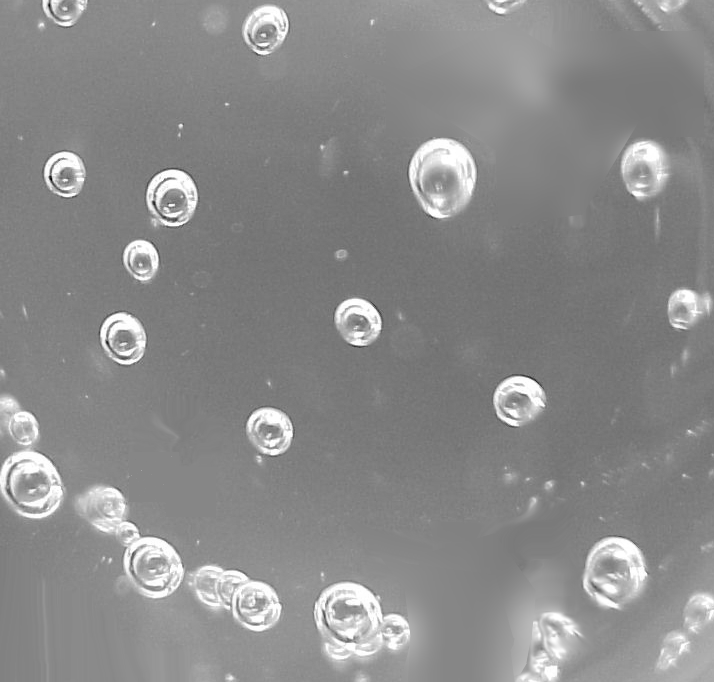
\includegraphics[width=\textwidth]{Assignment_1/input_images/bubbles.png}
        \caption{Input image \textit{"bubbles"}}
        \label{fig:orginalBubbles}
    \end{subfigure}
    \hfill
    \begin{subfigure}[t]{0.32\textwidth}
        \centering
        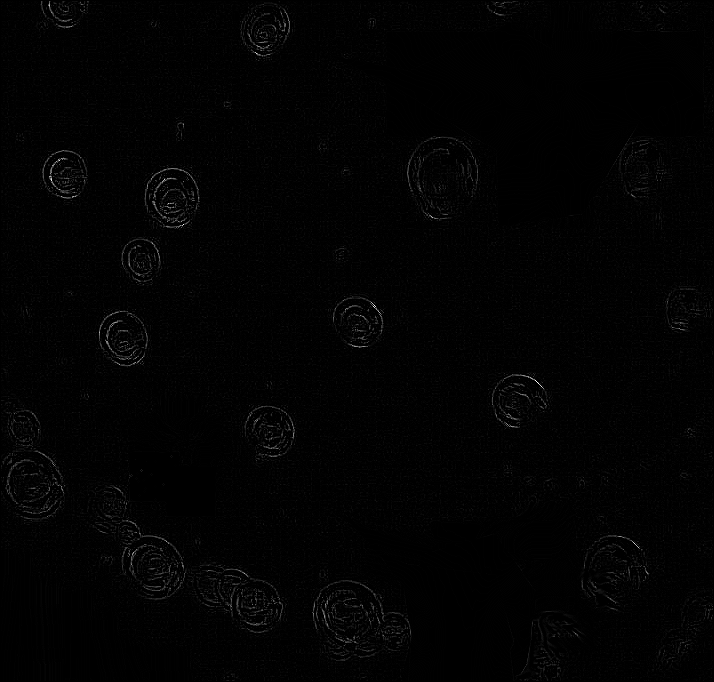
\includegraphics[width=\textwidth]{Assignment_1/output_images/filter_kevin.png}
        \caption{The output image using out own function \textit{IPfilter()}.}
        \label{fig:filterKevin}
    \end{subfigure}
    \hfill
    \begin{subfigure}[t]{0.32\textwidth}
        \centering
        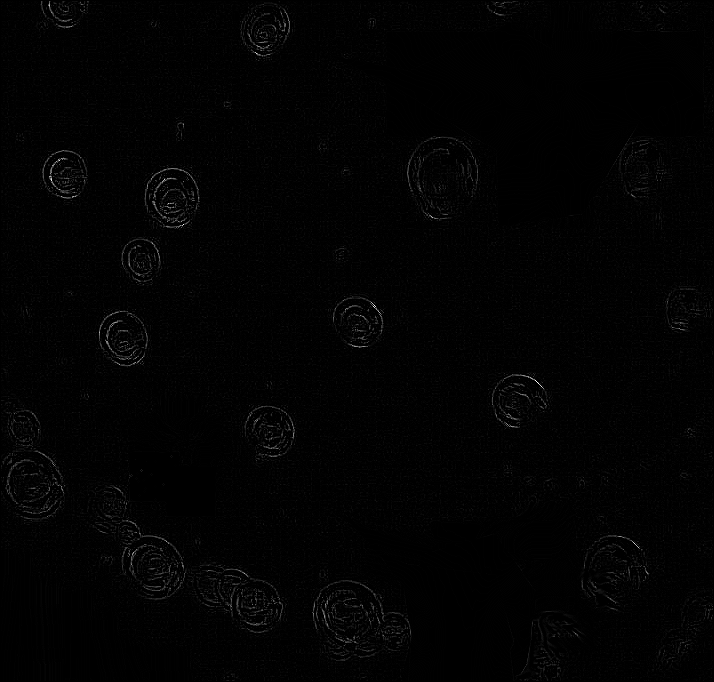
\includegraphics[width=\textwidth]{Assignment_1/output_images/filter_matlab.png}
        \caption{The output image using matlab's function \textit{filter2()}.}
        \label{fig:filterMatlab}
    \end{subfigure}
\end{figure}

To see if our implementation is working correctly we used the provided image \textit{"bubbles.tif"} and compared the result of using our function \textit{IPfilter} to the results of using the matlab function \textit{filter2}, as can be seen in Figure \ref{fig:filterResults}. Both Figure \ref{fig:filterKevin} and \ref{fig:filterMatlab} are exactly the same, thus showing our implementation is correct.

\subsection*{(b)}
For this part of the exercise we needed to implement the Laplacian (image) enhancement technique. This technique involves creating a Laplacian filter and then using the filter to enhance the original image. The Laplacian filter is the second derivative of the image, using a kernel. Formula \ref{eq:laplacian_filter} shows how this can be calculated for each pixel. It is easy to deduce here that the laplacian filter is simply a regular filter with a specific kernel applied. The book provides 4 different kernels that can be used. These are: 


\ding{118} Implementation: Listing~\ref{code:IPlaplacian}.

\subsection*{(c)}

\bibliographystyle{plain}
\bibliography{Assignment_1}

\appendix
\section{Code}
\subsection{Exercise 1}
\lstinputlisting[caption={IPscaling\_transformation.m: perform geometric transformations of \\the \textit{scaling} kind, given an affine transformation matrix or a scaling constant.}, label={code:IPscaling_transformation}]{Assignment_1/IPscaling_transformation.m}
\lstinputlisting[caption={IPinterpolate.m: interpolate an unknown pixel intensity value using\\ one of the supported methods.}, label={code:IPinterpolate}]{Assignment_1/IPinterpolate.m}
\subsubsection{Exercise 1 (a)}
\lstinputlisting[caption={IPdownsample.m: downsample images using \textsc{IPscaling\_transformation}.}, label={code:IPdownsample}]{Assignment_1/IPdownsample.m}
\subsubsection{Exercise 1 (c)}
\lstinputlisting[caption={IPupsample.m: upsample images using \textsc{IPscaling\_transformation}.}, label={code:IPupsample}]{Assignment_1/IPupsample.m}
\subsubsection{Exercise 1 (e)}
\lstinputlisting[caption={IPzoom.m: zoom images using \textsc{IPscaling\_transformation}.}, label={code:IPzoom}]{Assignment_1/IPzoom.m}
\subsection{Exercise 2}
\subsubsection{Exercise 2 (a)}
\lstinputlisting[caption={IPhistogram.m: construct an image's histogram.}, label={code:IPhistogram}]{Assignment_1/IPhistogram.m}
\subsubsection{Exercise 2 (b)}
\lstinputlisting[caption={IPhisteq.m: histogram equalization.}, label={code:IPhisteq}]{Assignment_1/IPhisteq.m}
\subsection{Exercise 3}
\subsubsection{Exercise 3 (a)}
\lstinputlisting[caption={IPfilter.m: image filter.}, label={code:IPfilter}]{Assignment_1/IPfilter.m}
\subsubsection{Exercise 3 (b)}
\lstinputlisting[caption={IPlaplacian.m: Laplacian enhancement technique.}, label={code:IPlaplacian}]{Assignment_1/IPlaplacian.m}
\end{document}
